\section{How threshold queries work}\label{s:threshold-reads}

\begin{figure}{r}{3in}
\vspace{-4em}
\begin{center}
  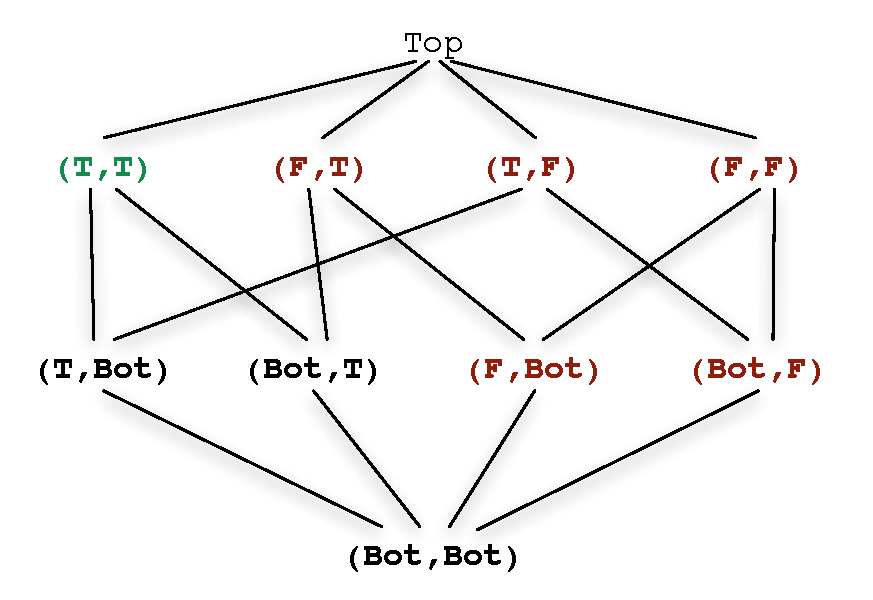
\includegraphics[width=3in]{chapter5/figures/parallel-and-take-2.pdf}
\end{center}
  \caption{Lattice of states that an \il{AndLV} can take on.  The five red
    states in the lattice correspond to a false result, and the one green to a true one.}
  \label{f:parallel-and}
\vspace{-2em}
\end{figure}

A \emph{threshold query} is a way of reading the contents of a
lattice-based data structure that allows only limited observations of
the state of the data structure.  It only returns a value when the
data structure's state meets a certain (monotonic) criterion, or
``threshold'', and the value returned is the same regardless of how
far above the threshold the data structure's state goes.  

By a \emph{lattice-based data structure}, we mean a data structure
whose possible states are elements of a lattice\footnote{We use
  ``lattice'' as a shorthand; formally, the ``lattice'' of states is a
  4-tuple $(D, \userleq, \bot, \top)$, where $D$ is a set, $\userleq$
  is a partial order on $D$, $\bot$ is $D$'s least element according
  to $\userleq$, $\top$ is $D$'s greatest element, and every two
  elements in $D$ have a least upper bound.  Hence $(D, \userleq,
  \bot, \top)$ is really a \emph{bounded join-semilattice} with a
  designated greatest element of $\top$.}, and that can only change
over time in a way that is inflationary with respect to the lattice.
Both CvRDTs~\cite{crdts,crdts-tr} and
LVars~\cite{LVars-paper,Freeze-paper} are examples of lattice-based
data structures.
%% A {threshold query} is defined over a lattice---specifically, any
%% changing value whose states are drawn from that lattice and increase
%% monotonically;
% increase monotonically within a partial order;
% occupy a lattice and monotonically increase, 
% (\eg{} Figure~\ref{f:parallel-and}),
%% this includes both LVars and each replica of a CvRDT.
%
%% The key is that threshold functions are undefined until the
%% value grows ``large enough'', after which
%% they return a specific value, and that result is invariant under
%% additional growth in the input.  That is, $f(x)=y \Rightarrow \forall{x'>x},\, f(x')=y$.
%% %
%% In practice, a call to a threshold query in an undefined state blocks
%% until it becomes defined.
%
%% We employ a useful class of threshold functions based on sets of
%% ``triggers'' which are pairwise incompatible (none above
%% another), enabling the threshold query to unblock and return the exact
%% element triggered.
% 
% 
In this section, we illustrate 
threshold queries with an example before
formally describing them in the context of CvRDTs.
% (Section~\ref{s:model}).

\subsection{An example: parallel ``and''}

Consider a lattice-based data structure that stores the result of a parallel logical ``and'' operation.
We will call this data structure an \emph{\il{AndLV}}.
For this example, we assume two inputs, called ``left'' and ``right'', 
each of which may be either \il{T} or \il{F}.
%
%% If this variable is replicated, then the write to the
%% left or right input may occur on any replica, but is eventually
%% propagated to other replicas.
%
% We also assume for the time being that we are \emph{not} dealing with
% a replicated data structure (or, equivalently, that we are dealing
% with only one replica); 
{To understand this example, it is sufficient to consider a single replica;}
in Section~\ref{s:model} we will go on to
discuss replication and communication between replicas.
%

\rn{Tweaked this because I didn't want to imply in any way that this
  example doesn't work with multiple replicas.  It's only for
  simplicity of exposition that we are holding off from talking about those.}
\lk{sounds good.}

We can represent the
states an \il{AndLV} can take on as pairs \il{(x,y)}, where each of
\il{x} and \il{y} are \il{T}, \il{F}, or \il{Bot}.  The \il{Bot}
value, short for ``bottom'', is the state in which no input has yet
been received, 
and so \il{(Bot,Bot)} is the least element of the lattice of
states that our \il{AndLV} can take on, shown in Figure~\ref{f:parallel-and}.
An additional state, which we call \il{Top},
is the greatest element of the lattice; it
represents the situation in which an error has occurred---if, for
instance, one of the inputs writes \il{T} and then later changes its
mind to \il{F}.

The result of the parallel ``and'' computation---if it completes
successfully---will be either \il{True} or \il{False}, but it might also
block indefinitely if not enough writes occur (say, if the left input
is \il{T} and the right input never arrives), or it could end in
an error state, discussed below.
%
{Each update to the lattice takes the form of a complete state,
  such as \il{(T,Bot)} to write the left input.}
\rn{This section didn't actually describe how write's happen - how is this?}
\lk{oops, fixed now.}

%
The lattice induces a \emph{join}, or least upper bound,
operation on 
pairs of states; for instance, the join of \il{(T,Bot)}
and \il{(Bot,F)} is \il{(T,F)}, and the join of \il{(T,Bot)} and
\il{(F,Bot)} is \il{Top} since the overlapping \il{T} and \il{F}
values conflict.
Importantly, whenever a write occurs, it updates the \il{AndLV}'s
state to the join of the incoming state and the current state.  (With
CvRDTs, this join is computed when replicas merge.  In this example,
though, we are dealing with only one replica, and updating to the join
of the new state and the current state is sufficient to ensure that
all writes are inflationary.)

\lk{TODO: show the Haskell code in an appendix?  I don't want to show
  it in the main part of the paper, not for this audience.}

\lk{TODO: Maybe we don't want typewriter font here at all,
  actually...}

\subsection{Threshold queries of an \il{AndLV}}

Given that we want the result of a threshold query to be a deterministic
function of the writes to a data structure---and not of the particular moment in
time the query is made---what sorts of observations are safe to make of an \il{AndLV}?
We cannot, for instance, test whether one or both inputs have been
written at a particular point in time, because the result will 
depend on how the test is interleaved with the writes.

Instead, we can describe a \emph{partial function} of the data
structure's state that is undefined for all states except those that
are at or above a certain \emph{threshold} in the lattice.
One way to describe such a function is to define a \emph{threshold
  set} of sets of ``activation'' states.  In the case of our
\il{AndLV}, one of these sets of activation states is the set of
states containing an \il{F}---that is, the set $\{
\textrm{\il{(F,Bot)}, \il{(Bot,F)}, \il{(F,T)}, \il{(T,F)},
  \il{(F,F)}} \}$.  The elements of this set are shown in red in
Figure~\ref{f:parallel-and}.  The other set of activation states
singleton set $\{ \textrm{\il{(T,T)}} \}$, shown in green in
Figure~\ref{f:parallel-and}.  Therefore the entire threshold set is
\[
\{ 
\{ \textrm{\il{(F,Bot)}, \il{(Bot,F)}, \il{(F,T)}, \il{(T,F)}, \il{(F,F)}} \},
\{ \textrm{\il{(T,T)}} \}
\}
\]
The semantics of a threshold query is as follows: if a data structure's state
reaches (or surpasses) any state or states in a particular set of activation
states, the threshold query returns \emph{the entire set} of
activation states, regardless of which of those activation states was reached. If
no state in any set of activation states has yet been reached, the
threshold query will \emph{block}; blocking corresponds to states on
which the partial function is undefined.

In the case of our \il{AndLV}, as soon as either input writes an
\il{F}, our threshold query will unblock and return the first set of
activation states, that is, $\{ \textrm{\il{(F,Bot)}, \il{(Bot,F)},
  \il{(F,T)}, \il{(T,F)}, \il{(F,F)}} \}$.  Hence \il{AndLV} has the
expected ``short-circuit'' behavior and does not have to wait for a
second input if the first input is \il{F}.  If, on the other hand, both
inputs write a \il{T}, the threshold query will unblock and return $\{
\textrm{\il{(T,T)}} \}$.

In a real implementation,
of course, the value returned from the query could be more meaningful
to the client---for instance, we could return \il{False}
instead of returning the set of activation states.  However,
doing so would only be a convenience, and the translation from $\{
\textrm{\il{(F,Bot)}, \il{(Bot,F)}, \il{(F,T)}, \il{(T,F)},
  \il{(F,F)}} \}$ to \il{False} could just as easily take place on the
client side.  In either case, the result returned from the
threshold query is the same regardless of \emph{which} of the activation
states caused it to unblock, and it is impossible for the client to
tell whether the actual state of the lattice is, say, \il{(T,F)} or
\il{(F,F)} or some other state containing \il{F}.

\subsection{Pairwise incompatibility}\label{subsec:pairwise-incompatibility}

In order for the behavior of a threshold query
to be deterministic, it must be unblocked by
a \emph{unique} set of activation states in the threshold set.  
We ensure this by
requiring that elements in a set of activation states must be
\emph{pairwise incompatible} with elements in every other set of
activation states.  That is, for all distinct sets of activation states $Q$
and $R$ in a given threshold set: $\forall q \in Q.~\forall r \in R.~q \sqcup r = \top$.
\lk{changed to inline math to save space.}
%% %
%% \[ \forall q \in Q.~\forall r \in R.~q \sqcup r = \top \]
%% %
In our \il{AndLV} example, there are two distinct sets of activation states, so if
we let $Q = \{ \textrm{\il{(T,T)}} \}$ and $R = \{
\textrm{\il{(F,Bot)}, \il{(Bot,F)}, \il{(F,T)}, \il{(T,F)},
  \il{(F,F)}} \}$, the least upper bound of \il{(T,T)} and $r$ must be
\il{Top}, where $r$ is any element of $R$.  We can easily verify that
this is the case.  Furthermore, since the lattice of states that an
\il{AndLV} can take on is finite, the join function can be verified to compute a
least upper bound.

Why is pairwise incompatibility necessary?  Consider the following
(illegal) ``threshold set'' that does not meet the pairwise
incompatibility criterion:
$ \{ \{ \textrm{\il{(F,Bot)}, \il{(Bot,F)}} \},  \{ \textrm{\il{(T,Bot)}, \il{(Bot,T)}} \} \} $.
\lk{changed to inline math to save space.}
%% \[
%% \{ 
%% \{ \textrm{\il{(F,Bot)}, \il{(Bot,F)}} \},
%% \{ \textrm{\il{(T,Bot)}, \il{(Bot,T)}} \}
%% \}
%% \]
A threshold query corresponding to this so-called threshold set will
unblock and return $\{ \textrm{\il{(F,Bot)}, \il{(Bot,F)}} \}$
as soon as a state containing an
\il{F} is reached, and $\{ \textrm{\il{(T,Bot)}, \il{(Bot,T)}} \}$
as soon as a state
containing a \il{T} is reached.  The trouble with such a threshold
query is that there exist states, such as \il{(F,T)} and \il{(T,F)},
that could unblock either set of activation states.  If the left input
writes \il{F} and the right input writes \il{T}, and these writes
occur in arbitrary order, then the threshold query will return a
nondeterministic result, depending on the order in which the two
writes arrive.  But with the original, pairwise-incompatible threshold
set we showed, the threshold query would deterministically return
\il{False}---although if the \il{T} arrived first, the query would
have to block until the \il{F} arrived, whereas if the \il{F} arrived
first, it could unblock immediately.  Hence threshold queries enforce
consistency at the expense of availability, but it is still possible
to do a ``short-circuit'' computation that unblocks as soon as an
\il{F} is written.

The threshold set mechanism we describe in this section is 
part of the LVars programming model discussed in
section~\ref{s:intro}; in fact, our \il{AndLV} example is precisely an
LVar~\cite{effectzoo}.  But the utility of threshold queries
is not limited to LVars.  In
the following sections, we review the basics of the CvRDT model from the work of
Shapiro \etal, then show how to add threshold queries to the CvRDT
model, and prove that they are strongly
consistent queries.

